	Beim letzten Mal hatten wir $\vec{A} (\vec{r}, t)$ quantisiert wie folgt:\marginpar{29.10.2015}
		\begin{align*}
			\hat{\vec{A}} (\vec{r})= \sqrt{\frac{\hbar}{2V}} ~c
			\sum_{\vec{k}, \lambda \in \{+ , i\}}
			\frac{1}{\sqrt{\omega_k}} \vec{\epsilon}_\lambda (\vec{k}) 
			\left\{ a_\lambda (\vec{k}) e^{i \vec{k} \vec{r}}
			+ a^\dagger_\lambda (\vec{k}) e^{-i \vec{k} \vec{r}}
			\right\}
		\end{align*}
	Wobei
		\begin{align*}
			a^\dagger_\lambda (\vec{k}) \ket{0} 
			&= \overbrace{\ket{\lambda, \vec{k}}}^{\mathclap{\text{Photon}}} \\
			a_\lambda (\vec{k}) \ket{0} &= 0 \\
			\vec{\epsilon}_\lambda (\vec{k}) &: \text{Polarisation} \\
			\hat{\vec{A}} (\vec{r}) &: \text{Operator (keine gewöhnliche Welle)} \\
			\hat{\vec{A}} (\vec{r}) \ket{0} &= \vec{A} (\vec{r})\ket{0} 
		\end{align*}
	D.h $\vec{A} (\vec{r})$ ist ein Eigenwert und enthält keine $a$ oder $a^\dagger$.
		\begin{empheq}[box=\boxed]{align*}
			H = \sum_{\vec{k}, \lambda} \hbar \omega_k
			\underbrace{a^\dagger_\lambda (\vec{k})~a_\lambda (\vec{k})}_{\substack{\text{Nummern oder} \\ \text{Teilchenoperator}}}
		\end{empheq}
	Wobei $\omega_k = c |\vec{k}|$ und kein $\frac{1}{2} \hbar \omega$ vorhanden ist, was damit zutun hat, dass wir nur den Grundzustand betrachten (glaube ich \^{}\^{}).
	
	Auf jeden Fall gilt für $n=1$:
		\begin{align*}
			H \ket{\lambda, \vec{k}} &= \hbar \omega_k \ket{\lambda , \vec{k}} \\
			\hat{\vec{p}} &= \hbar \vec{k} \ket{\lambda , \vec{k}} \\
			E = |\vec{p}| c &\curvearrowright H = |\hat{p}| c \\
			H \ket{0} (&= E_0 \ket{0} = 0 \ket{0} ) = 0
 		\end{align*}
 	Unendliches Volumen: 
	 	\begin{align*}
		 	\frac{1}{V} \sum_{\vec{k}} &\longmapsto \int \frac{\diff^3 k}{(2 \pi)^3}
		 	& \text{Wobei das~} \vec{k} \text{~so aufgebaut ist:~}k_i &= n_i \frac{2 \pi}{L}, n_i \in \mathds{Z}
	 	\end{align*} \marginpar{Bleibt die Frage, was $n_i$ sind}
		\begin{align*}
			V \delta_{\vec{k} , 0} &\longmapsto (2 \pi)^2 \delta^{(3)} (\vec{k}) \\
			a_\lambda (\vec{k}) &\longmapsto \frac{1}{\sqrt{\lambda}} 
			& &\text{(wegen Infrarot cutoff)}
		\end{align*} \marginpar{kA was das genau ist}
		\begin{align*}
			\vec{A} (\vec{r}) =
			\sqrt{\hbar} \int \frac{\diff^3 k}{(2 \pi)^3} \frac{c}{\sqrt{2 \omega_k}}
			\sum_\lambda \vec{\epsilon}_\lambda (\vec{k})
			\left\{ a_\lambda (\vec{k}) e^{i \vec{k} \vec{r}}
			+ a^\dagger_\lambda (\vec{k}) e^{-i \vec{k} \vec{r}}
			\right\}
		\end{align*}
	Wir betrachten ab jetzt den Fall: 
		\begin{figure*} [ht]
			\begin{center}
				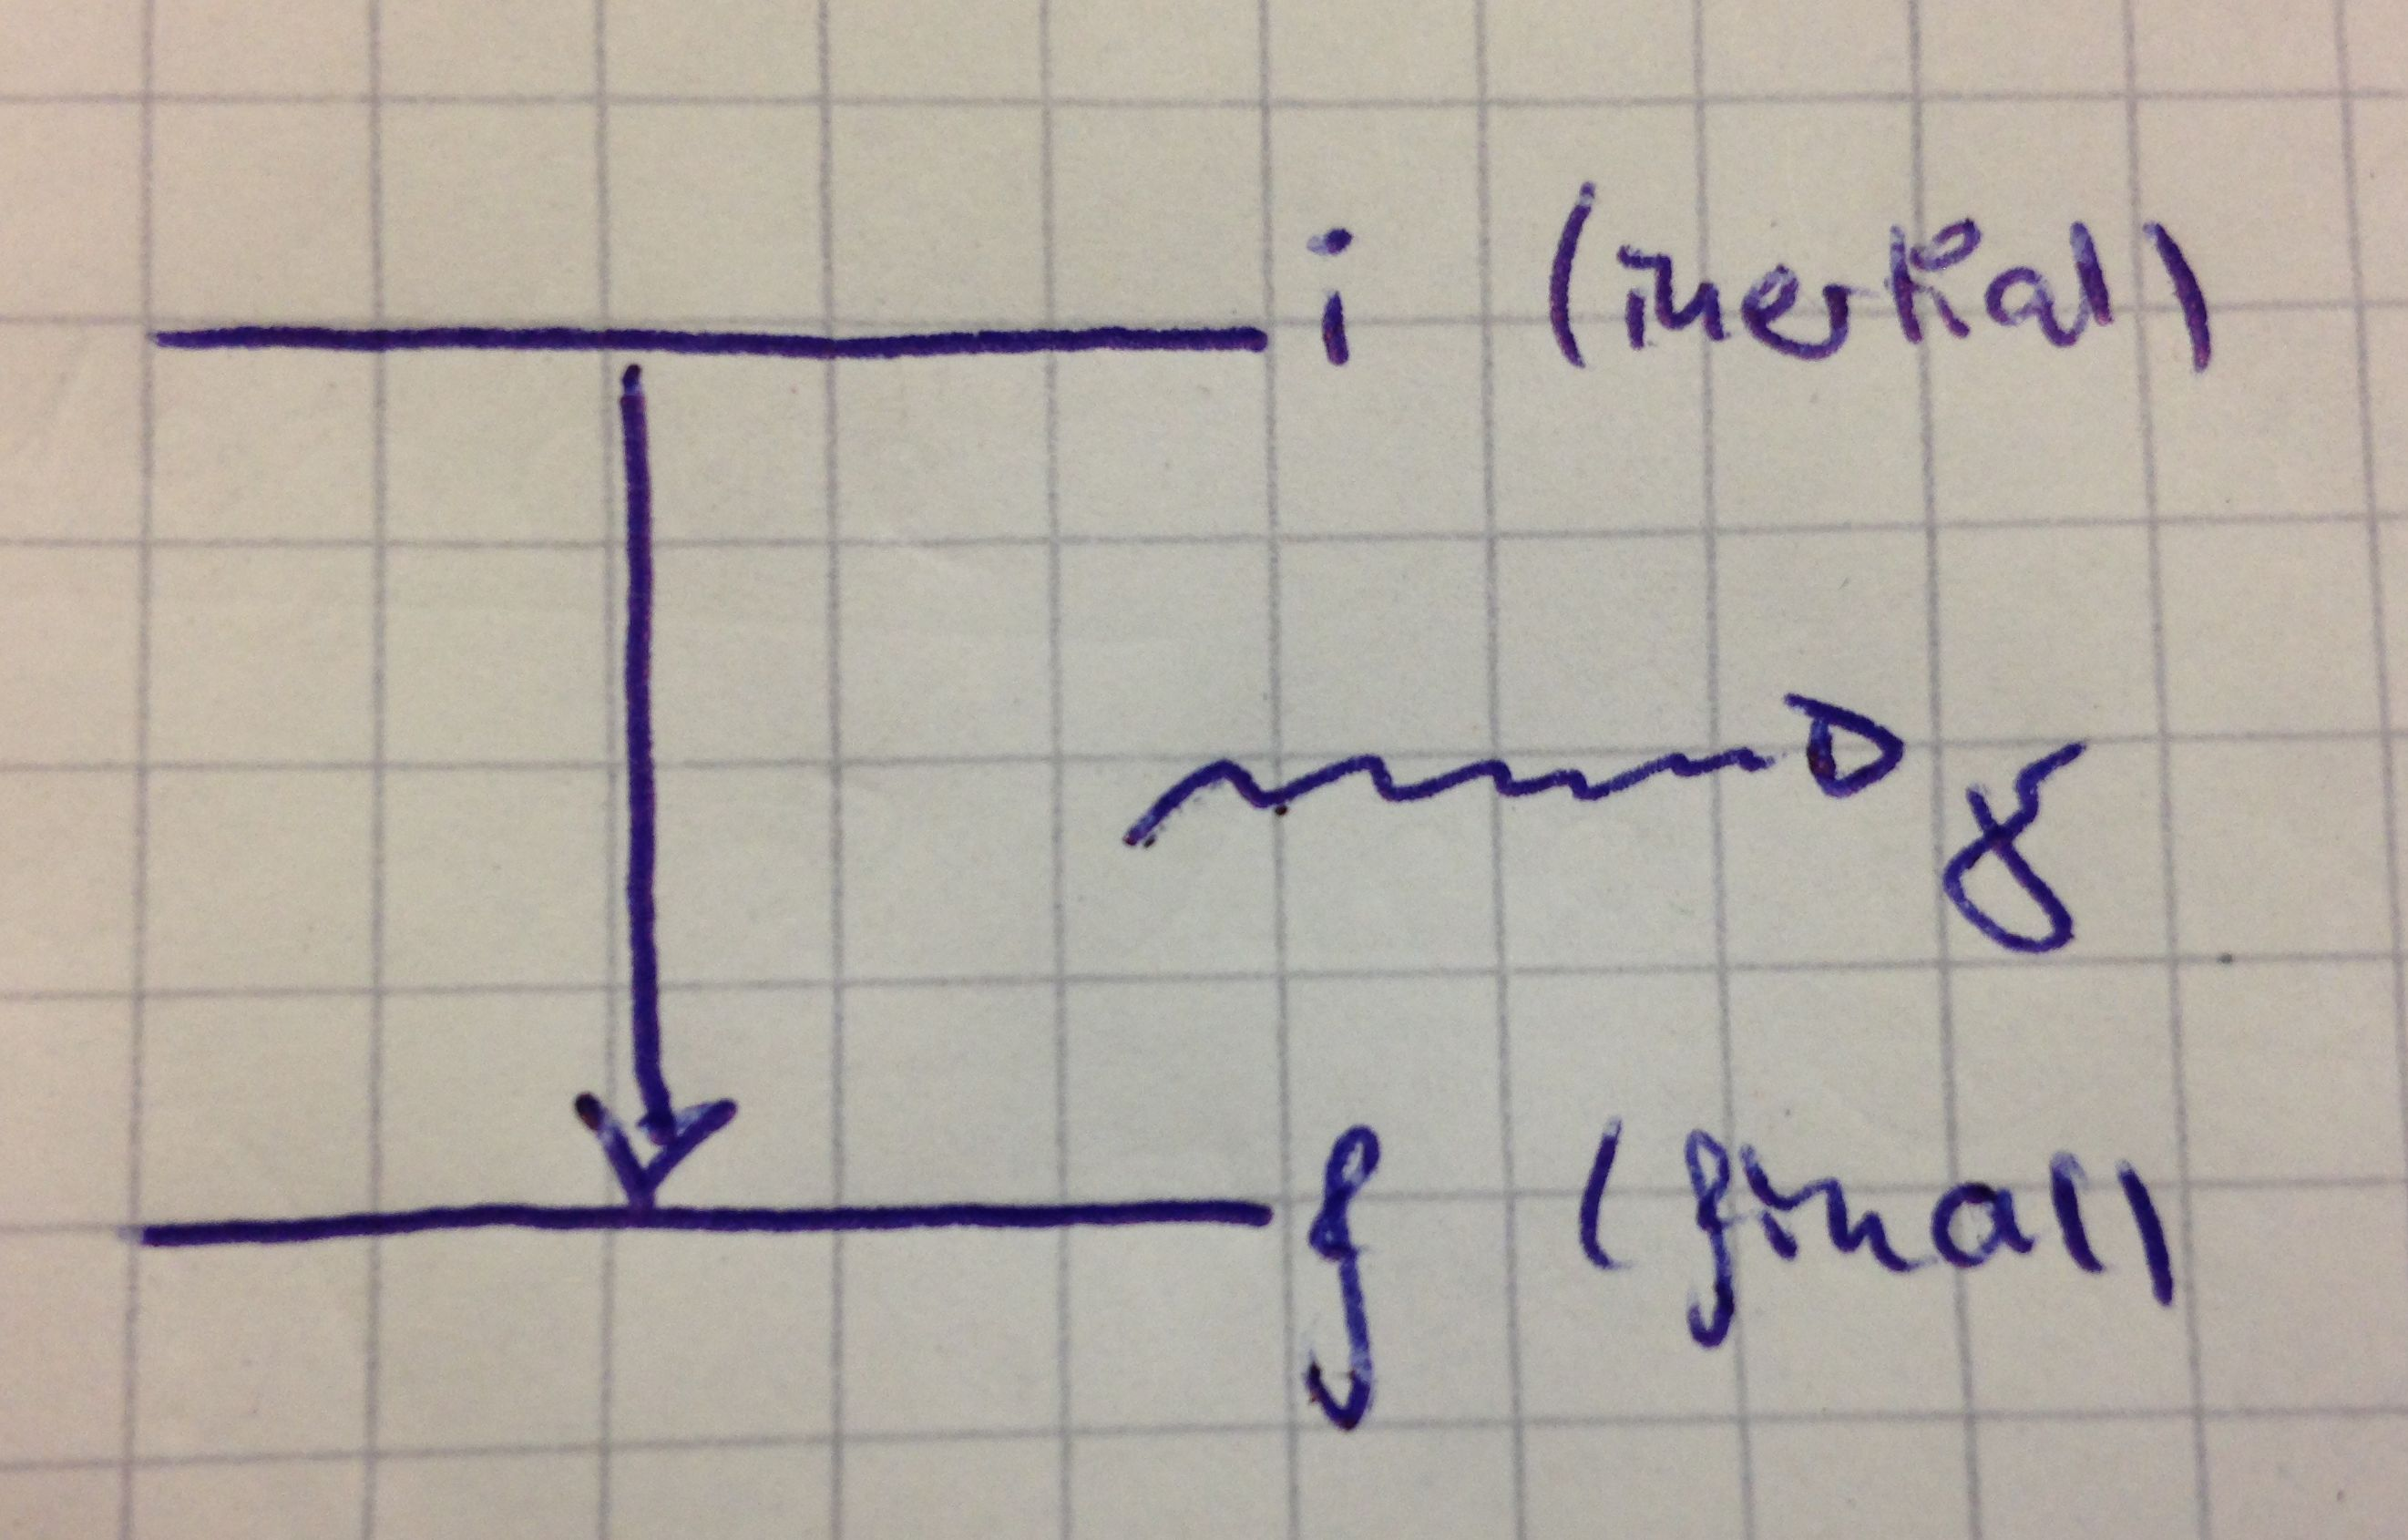
\includegraphics[width=10cm]{Bild2.jpg}
			\end{center}
		\end{figure*}
		\begin{align*}
			H &= H_e + H_\gamma & H_e &: \text{für Elektron}, ~ H_\gamma : \text{für Photon} \\
			H_e &= \underbrace{\frac{\vec{p}^2}{2 m_e} - e \Phi}_{\mathclap{H_e^0}}
			+ \frac{e \vec{A} \vec{p}}{m c}
			+ \frac{e^2}{2 m c^2} \vec{A}^2 &
			&\text{(Coulombeichung)}\\
			&= H_e^0 + H^1 + H^2 \\
			H_e^0 &= \frac{\vec{p}^2}{2 m} - Z \alpha \hbar c \frac{1}{r} & 
			Z &~\text{ist Kernladung},~ \alpha = \frac{e^2}{4 \pi \hbar c}\\
			H_e^0 \ket{n} &= E_n \ket{n} = \hbar \omega_n \ket{n} & 
			\ket{n} &~ \text{ist Elektronzustand}
		\end{align*}	
für ein H-Atom:
		\begin{align*}
			E_n &= - \frac{1}{2} (Z \alpha)^2 m c^2 \frac{1}{n^2}
			= \frac{1}{2} Z \alpha \hbar c \overbrace{\erw{r^{-1}}}^{\mathclap{\frac{Z}{a_B n^2}}}
			= - \frac{1}{2 n^2} \frac{Z^2 \alpha \hbar c}{a_B} &
			a_B &= \frac{\hbar}{m \alpha c} \\
			H_\gamma &= \int \frac{\diff^3 k}{(2 \pi)^3}
			\sum_{\lambda \in \{+,-\}} \hbar \omega_k
			~a_\lambda (\vec{k})~a^\dagger_\lambda (\vec{k})
		\end{align*}
	Anfangszustand: 
		\begin{align*}
			\ket{i} &= \ket{n(\ell, \ell_z); 0} = \ket{n} \otimes \ket{0}
		\end{align*}
	wobei im \underline{ersten Term} $n$ die Hauptquantenzahl ist, die $\ell$'s sind eigentlich immer da, aber aus Faulheit schreiben wir die fast nie mit, die $0$ bedeutet, dass wir kein Photon haben. Im \underline{zweiten Term} ist $\ket{n}$ der Zustand vom H-Atom und $\ket{0}$ der Zustand von der elektromagnetischen Welle.
	
	Endzustand:
		\begin{align*}
			\ket{f} &= \ket{m(\ell', \ell_z'); \vec{k}, \lambda} 
			= \ket{m} \otimes \ket{\vec{k}, \lambda}
		\end{align*} 
	Der Energieunterschied ist dann:\footnote{Ich habe den Betrag in $\omega_{mn}$ gesetzt, damit wir nicht mit Minuszeichen oder so durcheinander kommen.}
		\begin{align*}
			\Delta E &= E_f - E_i = \hbar 
			\underbrace{(|\omega_m - \omega_n)|}_{\mathclap{\omega_{mn}}} 
			+ \hbar c |\vec{k}| = \hbar (\omega_{mn} + \omega_k)
		\end{align*}
	Übergangsrate: 
		\begin{align*}
			W_{f \leftarrow i} &= 
			\int \frac{\diff^3 k}{(2 \pi)^3} \sum_\lambda
			\frac{2 \pi}{\hbar^2} \delta(\omega_{mn} + \omega_k)
			\left|\braket{f | H_e^1 + H_e^2 | i}\right|^2
		\end{align*}	
	Und $H_e^1 + H_e^2$ ist die Störung (Lösung für $H_e^0 + H_\gamma$ ist bekannt).
	
	Mit Hilfe von
		\begin{align*}
			\int \diff^3 k &= \int \diff k ~k^2 \int \diff \Omega_k
			= \frac{1}{c^3} \int \diff \omega_k ~\omega^2 \int \diff \Omega_k
		\end{align*}
	Können wir schreiben:
		\begin{align*}
			W_{f \leftarrow i} &= \int \diff \Omega_k 
			\frac{\omega_{mn}^2}{4 \pi^2 \hbar^2 c^3}
			\sum_\lambda 
			\left|\braket{f | H_e^1 + H_e^2 | i}\right|^2
		\end{align*}